%-----------------------------------------------------------------------------------------------------------------------------------------------%
%  The MIT License (MIT)
%
%  Copyright (c) 2015 Jan Küster
%
%  Permission is hereby granted, free of charge, to any person obtaining a copy
%  of this software and associated documentation files (the "Software"), to deal
%  in the Software without restriction, including without limitation the rights
%  to use, copy, modify, merge, publish, distribute, sublicense, and/or sell
%  copies of the Software, and to permit persons to whom the Software is
%  furnished to do so, subject to the following conditions:
%
%  THE SOFTWARE IS PROVIDED "AS IS", WITHOUT WARRANTY OF ANY KIND, EXPRESS OR
%  IMPLIED, INCLUDING BUT NOT LIMITED TO THE WARRANTIES OF MERCHANTABILITY,
%  FITNESS FOR A PARTICULAR PURPOSE AND NONINFRINGEMENT. IN NO EVENT SHALL THE
%  AUTHORS OR COPYRIGHT HOLDERS BE LIABLE FOR ANY CLAIM, DAMAGES OR OTHER
%  LIABILITY, WHETHER IN AN ACTION OF CONTRACT, TORT OR OTHERWISE, ARISING FROM,
%  OUT OF OR IN CONNECTION WITH THE SOFTWARE OR THE USE OR OTHER DEALINGS IN
%  THE SOFTWARE.
%
%
%-----------------------------------------------------------------------------------------------------------------------------------------------%


%============================================================================%
%
%  DOCUMENT DEFINITION
%
%============================================================================%

%we use article class because we want to fully customize the page and dont use a cv template
\documentclass[10pt,a4paper]{article}


%----------------------------------------------------------------------------------------
%  ENCODING
%----------------------------------------------------------------------------------------

%we use utf8 since we want to build from any machine
\usepackage[utf8]{inputenc}

%----------------------------------------------------------------------------------------
%  LANGUAGE
%----------------------------------------------------------------------------------------

\usepackage[italian]{babel}

%----------------------------------------------------------------------------------------
%  LOGIC
%----------------------------------------------------------------------------------------

% provides \isempty test
\usepackage{xifthen}

%----------------------------------------------------------------------------------------
%  FONT
%----------------------------------------------------------------------------------------

% some tex-live fonts - choose your own

%\usepackage[defaultsans]{droidsans}
%\usepackage[default]{comfortaa}
%\usepackage{cmbright}
\usepackage[default]{raleway}
%\usepackage{fetamont}
%\usepackage[default]{gillius}
%\usepackage[light,math]{iwona}
%\usepackage[thin]{roboto}

% set font default
\renewcommand*\familydefault{\sfdefault}
\usepackage[T1]{fontenc}

% more font size definitions
\usepackage{moresize}


%----------------------------------------------------------------------------------------
%  PAGE LAYOUT  DEFINITIONS
%----------------------------------------------------------------------------------------

%debug page outer frames
%\usepackage{showframe}


%define page styles using geometry
\usepackage[a4paper]{geometry}

% for example, change the margins to 2 inches all round
%Original \geometry{top=1.75cm, bottom=-.6cm, left=1.5cm, right=1.5cm}
\geometry{top=1.3cm, bottom=-.6cm, left=1.5cm, right=1.5cm}

%use customized header
\usepackage{fancyhdr}
\pagestyle{fancy}

%less space between header and content
\setlength{\headheight}{-5pt}


%customize entries left, center and right
%\lhead{}
%\chead{ \small{Riccardo Milani  $\cdot$ Mathematical Engineer $\cdot$  Italian, French  $\cdot$  \textcolor{sectcol}{\textbf{ricc.milani@gmail.com}}  $\cdot$ +33 6 43 34 16 23}}
%\rhead{}


%indentation is zero
\setlength{\parindent}{0mm}

%----------------------------------------------------------------------------------------
%  TABLE /ARRAY DEFINITIONS
%----------------------------------------------------------------------------------------

%for layouting tables
\usepackage{multicol}
\usepackage{multirow}

%extended aligning of tabular cells
\usepackage{array}

\newcolumntype{x}[1]{%
>{\raggedleft\hspace{0pt}}p{#1}}%
\newcolumntype{q}[1]{%
>{\raggedright\arraybackslash\hspace{0pt}}p{#1}}%


%----------------------------------------------------------------------------------------
%  GRAPHICS DEFINITIONS
%----------------------------------------------------------------------------------------

%for header image
\usepackage{graphicx}

%for floating figures
\usepackage{wrapfig}
\usepackage{float}
%\floatstyle{boxed}
%\restylefloat{figure}

%for drawing graphics
\usepackage{tikz}
\usetikzlibrary{shapes, backgrounds,mindmap, trees}

\usepackage{hyperref}
\hypersetup{%
    hidelinks,%
    colorlinks=false,%
    pdfauthor={Riccardo Milani},%
    pdftitle={CV Milani},%
    pdfdisplaydoctitle=true,%
    %pdfsubject={CV},
    pdfkeywords=CV,%
    %pdfpagemode=FullScreen,%
    %pdfmenubar=false,%
    %pdftoolbar=false,%
    pdflang=it-IT,%
    pdfcreator=LaTeX,%
}

\usepackage{fontawesome}

%----------------------------------------------------------------------------------------
%  Color DEFINITIONS
%----------------------------------------------------------------------------------------

\usepackage{color}

%accent color
\definecolor{sectcol}{RGB}{100,120,180}
\definecolor{lightsect}{RGB}{128,206,214}

%dark background color
\definecolor{bgcol}{RGB}{100,110,120}

%light background / accent color
\definecolor{softcol}{RGB}{225,225,225}


%============================================================================%
%
%
%  DEFINITIONS
%
%
%============================================================================%

%----------------------------------------------------------------------------------------
%   HEADER
%----------------------------------------------------------------------------------------

% remove top header line
\renewcommand{\headrulewidth}{0pt}

%remove botttom header line
\renewcommand{\footrulewidth}{0pt}

%remove pagenum
\renewcommand{\thepage}{}

%remove section num
\renewcommand{\thesection}{}

%----------------------------------------------------------------------------------------
%   ARROW GRAPHICS in Tikz
%----------------------------------------------------------------------------------------

% a six pointed arrow poiting to the left
\newcommand{\tzlarrow}{(0,0) -- (0.2,0) -- (0.3,0.2) -- (0.2,0.4) -- (0,0.4) -- (0.1,0.2) -- cycle;}

% include the left arrow into a tikz picture
% param1: fill color
%
\newcommand{\larrow}[1]
{\begin{tikzpicture}[scale=0.58]
   \filldraw[fill=#1!100,draw=#1!100!black]  \tzlarrow
 \end{tikzpicture}
}

% a six pointed arrow poiting to the right
\newcommand{\tzrarrow}{ (0,0.2) -- (0.1,0) -- (0.3,0) -- (0.2,0.2) -- (0.3,0.4) -- (0.1,0.4) -- cycle;}

% include the right arrow into a tikz picture
% param1: fill color
%
\newcommand{\rarrow}
{\begin{tikzpicture}[scale=0.7]
  \filldraw[fill=sectcol!100,draw=sectcol!100!black] \tzrarrow
 \end{tikzpicture}
}

\newif\ifcvtitle
\newif\ifcvsubtitle
\cvtitlefalse
\cvsubtitlefalse


%----------------------------------------------------------------------------------------
%  custom sections
%----------------------------------------------------------------------------------------

% create a coloured box with arrow and title as cv section headline
% param 1: section title
%
\newcommand{\cvsection}[1]
{
\colorbox{sectcol}{\mystrut \makebox[1\linewidth][l]{
\larrow{lightsect} \hspace{-8pt} \larrow{lightsect} \hspace{-8pt} \larrow{lightsect} \textcolor{white}{\textbf{#1}}\hspace{4pt}
}}\\
}

\newcommand{\cvsubsection}[1]
{
\mystrut \makebox[1\linewidth][l]{
\larrow{bgcol} \hspace{-8pt} \larrow{bgcol} \hspace{-8pt} \larrow{bgcol} \textcolor{sectcol}{\textbf{#1}}
}\\
\vspace{-6pt}
\textcolor{softcol}{\hrule}
}

%create a coloured arrow with title as cv meta section section
% param 1: meta section title
%
\newcommand{\metasection}[2]
{
\begin{tabular*}{1\textwidth}{p{2.4cm} p{11cm}}
\larrow{bgcol}  \normalsize{\textcolor{sectcol}{#1}}&#2\\[12pt]
\end{tabular*}
}

%----------------------------------------------------------------------------------------
%   CV EVENT
%----------------------------------------------------------------------------------------

% creates a stretched box as cv entry headline followed by two paragraphs about
% the work you did
% param 1:  event time i.e. 2014 or 2011-2014 etc.
% param 2:  event name (what did you do?)
% param 3:  institution (where did you work / study)
% param 4:  what was your position
% param 5:  some words about your contributions
%
\newcommand{\cvevent}[5]
{
\vspace{8pt}
  \begin{tabular*}{1\textwidth}{p{2.3cm} p{7.8cm} x{6.9cm}} %10.8 3.9
 \textcolor{bgcol}{#1}& \textbf{#2} & \vspace{2.5pt}\textcolor{sectcol}{#3}

  \end{tabular*}
\vspace{-12pt}
\textcolor{softcol}{\hrule}
\vspace{6pt}
  \begin{tabular*}{1\textwidth}{p{2.3cm} q{15.2cm}}
&\larrow{bgcol} {#4}\\[3pt]
&\larrow{bgcol} {#5}\\[6pt]
  \end{tabular*}

}

% creates a stretched box as
\newcommand{\cveventmeta}[2]
{
  \mbox{\mystrut \hspace{87pt}\textit{#1}}\\
  #2
}

%----------------------------------------------------------------------------------------
% CUSTOM STRUT FOR EMPTY BOXES
%----------------------------------------- -----------------------------------------------
\newcommand{\mystrut}{\rule[-.3\baselineskip]{0pt}{\baselineskip}}

%----------------------------------------------------------------------------------------
% CUSTOM
%----------------------------------------------------------------------------------------
% Lorem
\newcommand{\lorem}
{Lorem ipsum dolor sit amet, consectetur adipiscing elit. Donec a diam lectus.}

% Code_Saturne
\newcommand{\cs}{{\fontfamily{ppl}\fontshape{it}\selectfont Code\_Saturne}}

\title{CV - Ita}

%============================================================================%
%
%
%
%  DOCUMENT CONTENT
%
%
%
%============================================================================%
\begin{document}


%use our custom fancy header definitions
\pagestyle{fancy}


%---------------------------------------------------------------------------------------
%  TITLE HEADLINE
%----------------------------------------------------------------------------------------
\vspace{-20.55pt}

% use this for multiple words like working titles etc.
%\hspace{-0.25\linewidth}\colorbox{bgcol}{\makebox[1.5\linewidth][c]{\hspace{46pt}\HUGE{\textcolor{white}{\textsc{Jan Küster}} } \textcolor{sectcol}{\rule[-1mm]{1mm}{0.9cm}} \parbox[b]{5cm}{   \large{ \textcolor{white}{{IT Consultant}}}\\
% \large{ \textcolor{white}{{Resume}}}}
%}}

% use this for single words, e.g. CV or RESUME etc.
\hspace{-0.25\linewidth}\colorbox{bgcol}{\makebox[1.5\linewidth][c]{\href{https://cermics.enpc.fr/~milanir/}{\HUGE{\textcolor{white}{Riccardo \textbf{\textsc{Milani}}}} } \textcolor{lightsect}{\rule[-1mm]{1mm}{0.9cm}} \HUGE{\textcolor{white}{\textsc{CV}} } }}

\vspace{2px}
\center{%
 \ifcvtitle{Ingegnere Matematico $\cdot$} \fi%
 Italiano, Francese $\cdot$ %\faFlag~
 15/01/1991 $\cdot$ %
 Lecco $\cdot$ %
 \href{mailto:ricc.milani@gmail.com}{\textcolor{sectcol}{\textbf{ricc.milani@gmail.com}}} $\cdot$ %\faEnvelope
 {+33 7 83 93 34 47} $\cdot$ %\faPhone or \faMobilePhone\footnotesize
 \textcolor{sectcol}{\faLinkedinSquare\href{www.linkedin.com/in/milanir}{\bfseries/in/milanir}} $\cdot$ %
 \faGithub\href{www.github.com/RiMillo}{/RiMillo}% $\cdot$ %
}
\vspace{2px}
\center{\huge{\textbf{\textcolor{sectcol}{%
% Title
\ifcvtitle%
  PhD in Matematica Applicata / CFD%
\else%
  Ingegnere Matematico%
\fi
}}}}%
%\vspace{-2px}
% ================
% Subtitle
\ifcvsubtitle%
  \center{\large{\textcolor{bgcol}{A partire da estate/autunno 2017}}}%
\else%
  \vspace*{2px}
\fi
\vspace*{4px}%
% ================
\vspace{4px}%
%
%----------------------------------------------------------------------------------------
%  HEADER IMAGE
%----------------------------------------------------------------------------------------

%\begin{figure}[H]
%\begin{flushright}
  %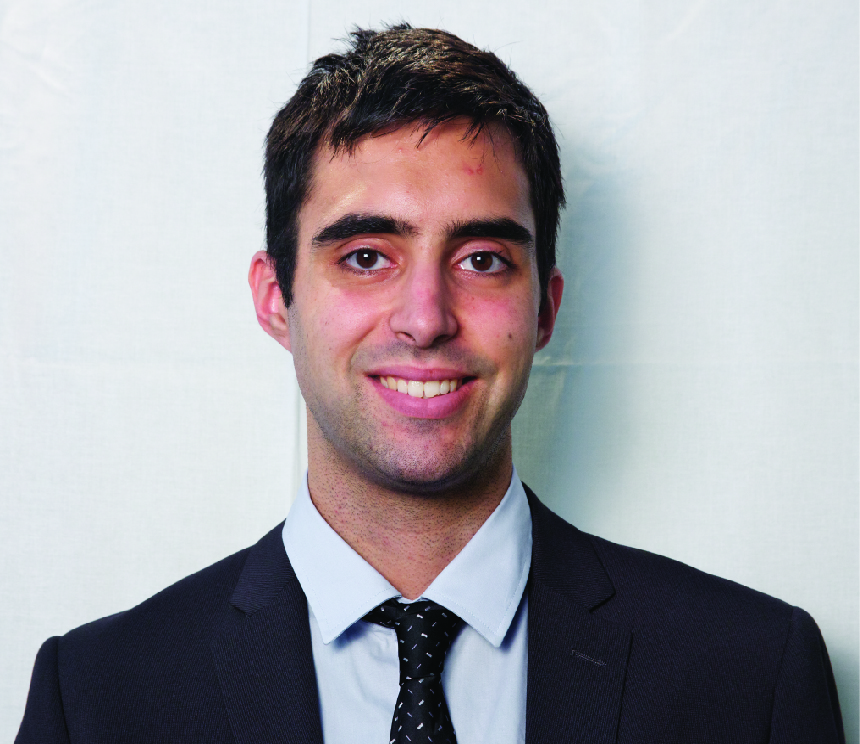
\includegraphics[trim= 320 130 460 210,clip,width=0.2\linewidth]{Foto_Smart.jpg}  %trimming relative to image size!
    %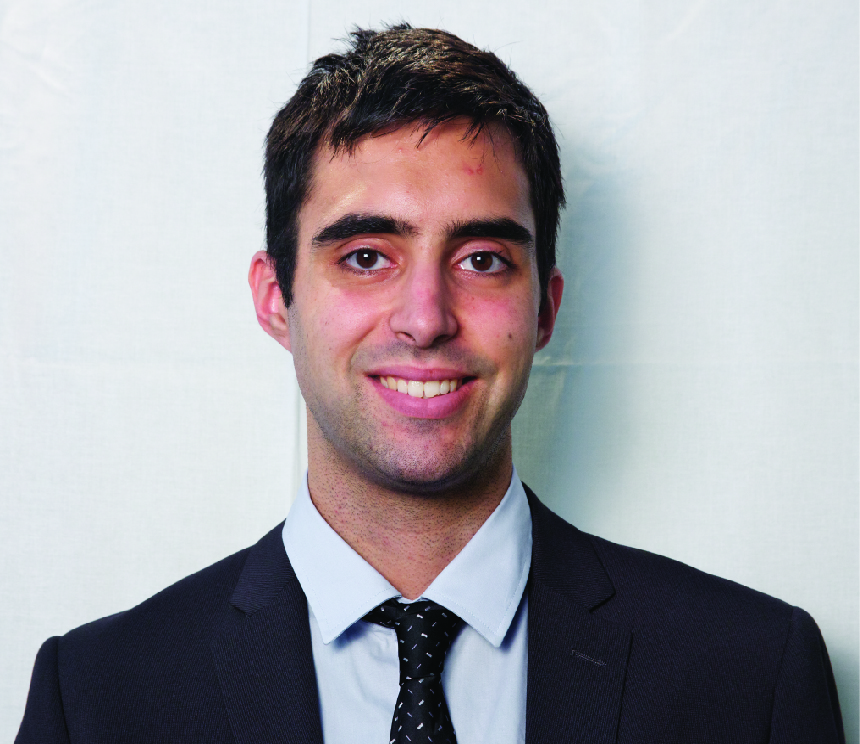
\includegraphics[width=0.2\linewidth]{Foto_Smart.jpg}
%\end{flushright}
%\end{figure}

%---------------------------------------------------------------------------------------
%  QR CODE (optional)
%----------------------------------------------------------------------------------------
%\vspace{-136pt}
%\hspace{0.75\linewidth}
%
\includegraphics[width=103pt]{qrcode}
%\normalsize
%\vspace{88pt}

%---------------------------------------------------------------------------------------
%  META SECTION
%----------------------------------------------------------------------------------------

%\vspace{-114pt}

%\metasection{Status:}{M.Sc. Digital Media, IT Consultant at We4IT Bremen}
%\metasection{Fields:}{Project Management, Software Development, Scrum, Usability}
%\metasection{Prefers:}{JS, Java, XPages, Flex / AIR, Processing, Git, Eclipse}
%\metasection{Activities:}{Global Game Jam, Sound Engineering, Blender, Martial Arts}

%\vspace{6pt}

%---------------------------------------------------------------------------------------
%  SUMMARAY (optional)
%----------------------------------------------------------------------------------------

%\cvsection{Summary}\\
%Digital media graduate with four years project experience in the field of technology based assessment. Specialized in development of test-scenario engines and innovative, rich media item formats. Master studies focused on teams from different disciplines and cultural backgrounds on solutions for complex problems.  Prior knowledge has been collected in he field of usability / accessibility during bachelor studies.\\

%============================================================================%
%
%  CV SECTIONS AND EVENTS (MAIN CONTENT)
%
%============================================================================%

%---------------------------------------------------------------------------------------
%  EDUCATION SECTION
%--------------------------------------------------------------------------------------
\cvsection{Formazione}

\cvevent{Dal 2017}%
        {Dottorando in matematica applicata}%
        {\'Ecole des Ponts ParisTech - EDF R\&D}%
        {\noindent Schemi CDO per le equazioni non-stazionarie di Navier--Stoker per un fluido incopressibile}%
        {Tutor: Ern Alexandre (CERMICS) e Bonelle J\'er\^ome (EDF R\&D)}%

\cvevent{2015 - 2017}%
        {Laurea Magistrale}%
        {Politecnico di Milano}%
        {Ingegneria Matematica, specializzazione: Scienze Computazionali per l'Ingegneria}%
        {Voto di Laurea: 110 e Lode/110}

%\textcolor{softcol}{\hrule}

%
\cvevent{2013 - 2017}%
        {Ciclo  dell'Ingegner \textit{Polytechnicien}}%
        {École polytechnique}%
        {Palaiseau, Francia. Equivalente a BSc e MSc}%
        {Specializzazione: Matematica Applicata -- EDP}

%\textcolor{softcol}{\hrule}

%
\cvevent{2010 - 2015}%
        {Laurea Triennale}%
        {Politecnico di Milano}%
        {Ingegneria Matematica. Voto di Laurea: 110 e Lode/110}%
        {Premio "Miglior Matricola" (2010) dopo i risultati del test d'ingresso e degli esami del primo semestre}

%---------------------------------------------------------------------------------------
%  EXPERIENCE
%----------------------------------------------------------------------------------------
\cvsection{Esperienze professionali}

%
\cvevent{09/'16-02/'17}%
        {Stage di Ricerca, 6 mesi}%
        {EDF R\&D, Chatou}{Sviluppo e analisi numerica di un metodo HHO per i problemi di diffusione anisotropa}%
        {Integrazione nel software industriale \cs{}; parallelizzazione con OpenMP}

%\textcolor{softcol}{\hrule}

%
\cvevent{03-08/2015}%
        {Stage di Ricerca, 5 mesi}%
        {US ESI R\&D, San Diego}%
        {Primi passi verso lo sviluppo di un nuovo sistema per un calcolo rapido della risposta vibro-acustica di un sistema}{Convalida con simulazioni}

%\textcolor{softcol}{\hrule}

%
\cvevent{08/2014}%
        {Stage Estivo}%
        {VTB Bank, Inkutsk}%
        {Foreign Exchange Control Group}%
        {Aiuto nella preparazione e convalida finale di contratti internazionali, gestione d'archivio}

\vspace{12pt}
\begin{minipage}{.48\linewidth}
\begin{flushleft}
\cvsubsection{Competenze informatiche}
\vspace{6pt}
\begin{tabular*}{1\linewidth}{l l}
&     \larrow{bgcol} \textbf{Buone}: \texttt{C}/\texttt{C++}, OpenMP, MPI, \LaTeX, sistemi Unix,\\[3pt]
&       MATLAB/Scilab, Git/SVN, \cs{}, Office\\[3pt]
&     \larrow{bgcol} \textbf{Basiche}: Python, shell script, FreeFem\texttt{++}, Fortran,\\[3pt]
&       Salome, Java, R
  \end{tabular*}
\end{flushleft}
\end{minipage}
\hfill
\begin{minipage}{.48\linewidth}
\begin{flushright}
\cvsubsection{Lingue}
\vspace{6pt}
\begin{tabular*}{1\linewidth}{l l l}
&     \larrow{bgcol} \textbf{Italiano}: &Madrelingua\\[3pt]
&     \larrow{bgcol} \textbf{Inglese}:  &Fluente, certificazione FCE, B2\\[3pt]
&     \larrow{bgcol} \textbf{Francese}: &Fluente, certificazione TCF, C1\\[3pt]
&     \larrow{bgcol} \textbf{Russo}:    &Livello base\\[3pt]
  \end{tabular*}
\end{flushright}
\end{minipage}

\bigskip

\begin{minipage}{.48\linewidth}
\begin{flushleft}
\cvsubsection{Attività extracurriculari}
\vspace{6pt}
\begin{tabular*}{1\textwidth}{l l}
&     \larrow{bgcol} Gestione di un dormitorio di studenti ('15) \\[3pt]
&     \larrow{bgcol} Tesoriere dell'AIM ('16)\\[3pt]
&     \larrow{bgcol} Rappresentante dei dottorandi EDF-MFEE ('18-'20) \\[3pt]
&     \larrow{bgcol} Running (maratona di Parigi '19)\\[3pt]
  \end{tabular*}
\end{flushleft}
\end{minipage}
\hfill
\begin{minipage}{.48\linewidth}
\begin{flushright}
\cvsubsection{Volontariato e altri Interessi}
\vspace{6pt}
\begin{tabular*}{1\linewidth}{l l}
&     \larrow{bgcol} Campi estivi (Kenya '10, '11; Ruanda '17)\\[3pt]
&     \larrow{bgcol} Membro di Smileland, che sostiene \\[3pt]
&       un villaggio di orfani in Congo\\[3pt]
&     \larrow{bgcol} Insegnamento di italiano per i profughi ('15-'16)\\[3pt]
  \end{tabular*}
\end{flushright}
\end{minipage}




%-------------------------------------------------------------------------------------------------
%  ARTIFICIAL FOOTER (fancy footer cannot exceed linewidth)
%--------------------------------------------------------------------------------------------------

\null
\vspace*{\fill}
%\hspace{-0.25\linewidth}\colorbox{bgcol}{\makebox[1.5\linewidth][c]{\mystrut \small \textcolor{white}{www.jankuester.com} $\cdot$ \textcolor{white}{github.com/jankapunkt}}}




%============================================================================%
%
%
%
%  DOCUMENT END
%
%
%
%============================================================================%
\end{document}
